\documentclass[12pt]{article}
\usepackage[a4paper, margin=1in]{geometry}
\usepackage{endnotes}
\usepackage{amsmath}
\usepackage{graphicx}
\usepackage{listings}
\usepackage{float} % For placing figures.
\usepackage[bottom]{footmisc}
\usepackage{tikz}

\setlength{\parskip}{0.5em}
\setlength{\parindent}{1em}

\def\code#1{\texttt{#1}}
\def\checkmark{\tikz\fill[scale=0.4](0,.35) -- (.25,0) -- (1,.7) -- (.25,.15) -- cycle;} 

% FILL IN TITLE AND AUTHOR
\title{
{CS3102 P2: Practical Report}\\
{\large Reliable Data Transfer Using UDP}\\
{
\includegraphics[width=80mm]{images/university-logo.png}}
}
\author{190010906}
\date{01 April 2022}

\begin{document}

\maketitle

\newpage

\section{Introduction}

Reliable Data Transport (RDT) is a unicast, connection-oriented protocol designed to provide reliable, ordered data transfer. This report will cover the detail, analyse and evaulate the design and implementation of RDT.

\section{Design}

Given the scope of the practical, simplicity was the main goal when designing the RDT protocol. This section will discuss design decisions and rationale behind them. The two attempted extension features, checksums and adaptive re-transmission timeouts,  are also detailed here.

\subsection{Packet Structure}

RDT packets (see Figure~\ref{fig:packet}) are composed of a constant 12 byte header and an optional data segment. The size of the data segment ranges from 0 to 1300 bytes, with 1300 bytes used as the maximum size so as to allow testing with \code{slurpe-3} without issue. Given that the TCP Maximum Segment Size (MSS)~\cite{rfc793} is generally 1500 bytes, this was considered a reasonable choice. Larger packet sizes may also lead to fragmentation at the IP Layer, which was undesirable.

\begin{figure}[h]
\begin{verbatim}
+-+-+-+-+-+-+-+-+-+-+-+-+-+-+-+-+-+-+-+-+-+-+-+-+-+-+-+-+-+-+-+-+
|   Header (12 Bytes)   |         Data (0 - 1300 Bytes)         |
+-+-+-+-+-+-+-+-+-+-+-+-+-+-+-+-+-+-+-+-+-+-+-+-+-+-+-+-+-+-+-+-+
\end{verbatim}
\caption{RDT Packet Structure}\label{fig:packet}
\end{figure}

The RDT header (see Figure~\ref{fig:header}) is comprised of the following fields: a 32-bit \code{sequence} field, used for keeping track of the number of bytes sent by the client; a 16-bit \code{type} field, used to denote the packet function; a 16-bit \code{checksum} field, calculated over the header and data segment to detect bit-errors; a 16-bit \code{size} field denoting the size of the data segment (in bytes); and a 16-bit \code{padding} field to ensure 32-bit word alignment.

Several factors influenced the RDT header design. As file sizes are often calculated as 32-bit integers (such as bythe C library function \code{ftell}), a 32-bit \code{sequence} field was required to support the transmission of large files/amounts of data. For checksums, the given implentation of the IPv4 header checksum used returns a \code{uint16\char`_t} value, thus necessitating a 16-bit field. As a maximum data segment size of 1300 bytes was required, at least 11 bits were required for the \code{size} field, however 16 bits were used for alignment. For the remaining \code{type} and \code{padding} fields, there were no other considerations for field size other than 32-bit alignment. 

\begin{figure}
\begin{center}
\begin{verbatim}
 0                   1                   2                   3  
 0 1 2 3 4 5 6 7 8 9 0 1 2 3 4 5 6 7 8 9 0 1 2 3 4 5 6 7 8 9 0 1
+-+-+-+-+-+-+-+-+-+-+-+-+-+-+-+-+-+-+-+-+-+-+-+-+-+-+-+-+-+-+-+-+
|                            Sequence                           |
+-+-+-+-+-+-+-+-+-+-+-+-+-+-+-+-+-+-+-+-+-+-+-+-+-+-+-+-+-+-+-+-+
|              Type             |            Checksum           |
+-+-+-+-+-+-+-+-+-+-+-+-+-+-+-+-+-+-+-+-+-+-+-+-+-+-+-+-+-+-+-+-+
|              Size             |            Padding            |
+-+-+-+-+-+-+-+-+-+-+-+-+-+-+-+-+-+-+-+-+-+-+-+-+-+-+-+-+-+-+-+-+
\end{verbatim}
\end{center}
\caption{RDT Header}\label{fig:header}
\end{figure}

A single \code{type} field was chosen, rather than a set TCP-style flags, for simplicity. Given the minimal nature of the RDT protocol, it was faster simpler to enumerate all packet types (see below), rather than testing multiple flags.

The type field supports the following types: \code{SYN} (0) and \code{SYN ACK} (1), used for the connection handshake; \code{DATA} (2) and \code{ACK} (3), used for sending and acknowledging data segments; \code{FIN} (4) and \code{FIN ACK} (5), used for graceful connection termination; and \code{RST} (6), used for abrupt connection termination.

\subsection{Connection Management}

The operation of the RDT protocol can be modelled by the FSM in Figure~\ref{fig:fsm}. For connection management, a two-way handshake is used. As RDT only supports uni-directional communication, a two-way handshake (see Figure~\ref{fig:timeline}) is adequate for establishing and terminating connections. Adaptive re-transmission timeouts are used in both the handshakes and transmission of data segments.

During handshakes, timeouts are used, with an initial RTO value of 200ms. This is doubled successively (Section~\ref{sec:RTO}). After 5 timeouts, the client with aborts with an \code{RST} to prevent clients waiting on unavailable hosts or a dropped \code{FIN ACK}.

\subsection{Data Transfer}

RDT uses an Idle-RQ mechanism for sending data segments, and will wait for acknowledgement of each sent segment. If the sender receives an \code{ACK} with a sequence number that is greater than expected or an RTO is triggered, it will retransmit the same packet. If it receives an \code{ACK} with a sequence number lower than expected, it will retransmit from that segment as it assumes a data segment has been dropped or corrupted\dots

For the handshake, a random sequence number is chosen to prevent `old' or `stale' packets from causing errors, and to reduce predictability that could be exploited. The method for generating initial sequence numbers is pseudo-random and not cryptograhically secure. 

\subsection{Adaptive RTO}\label{sec:RTO}
As an extension, adaptive re-transmission timeouts using measured RTT has been implemented. RDT's adaptive RDT is modelled on TCP's Retranmission Timer~\cite{rfc6298}\textsuperscript{1}, with the same initial RTO of 1s and maximum of 60s.

\begin{figure}[H]
\begin{center}
    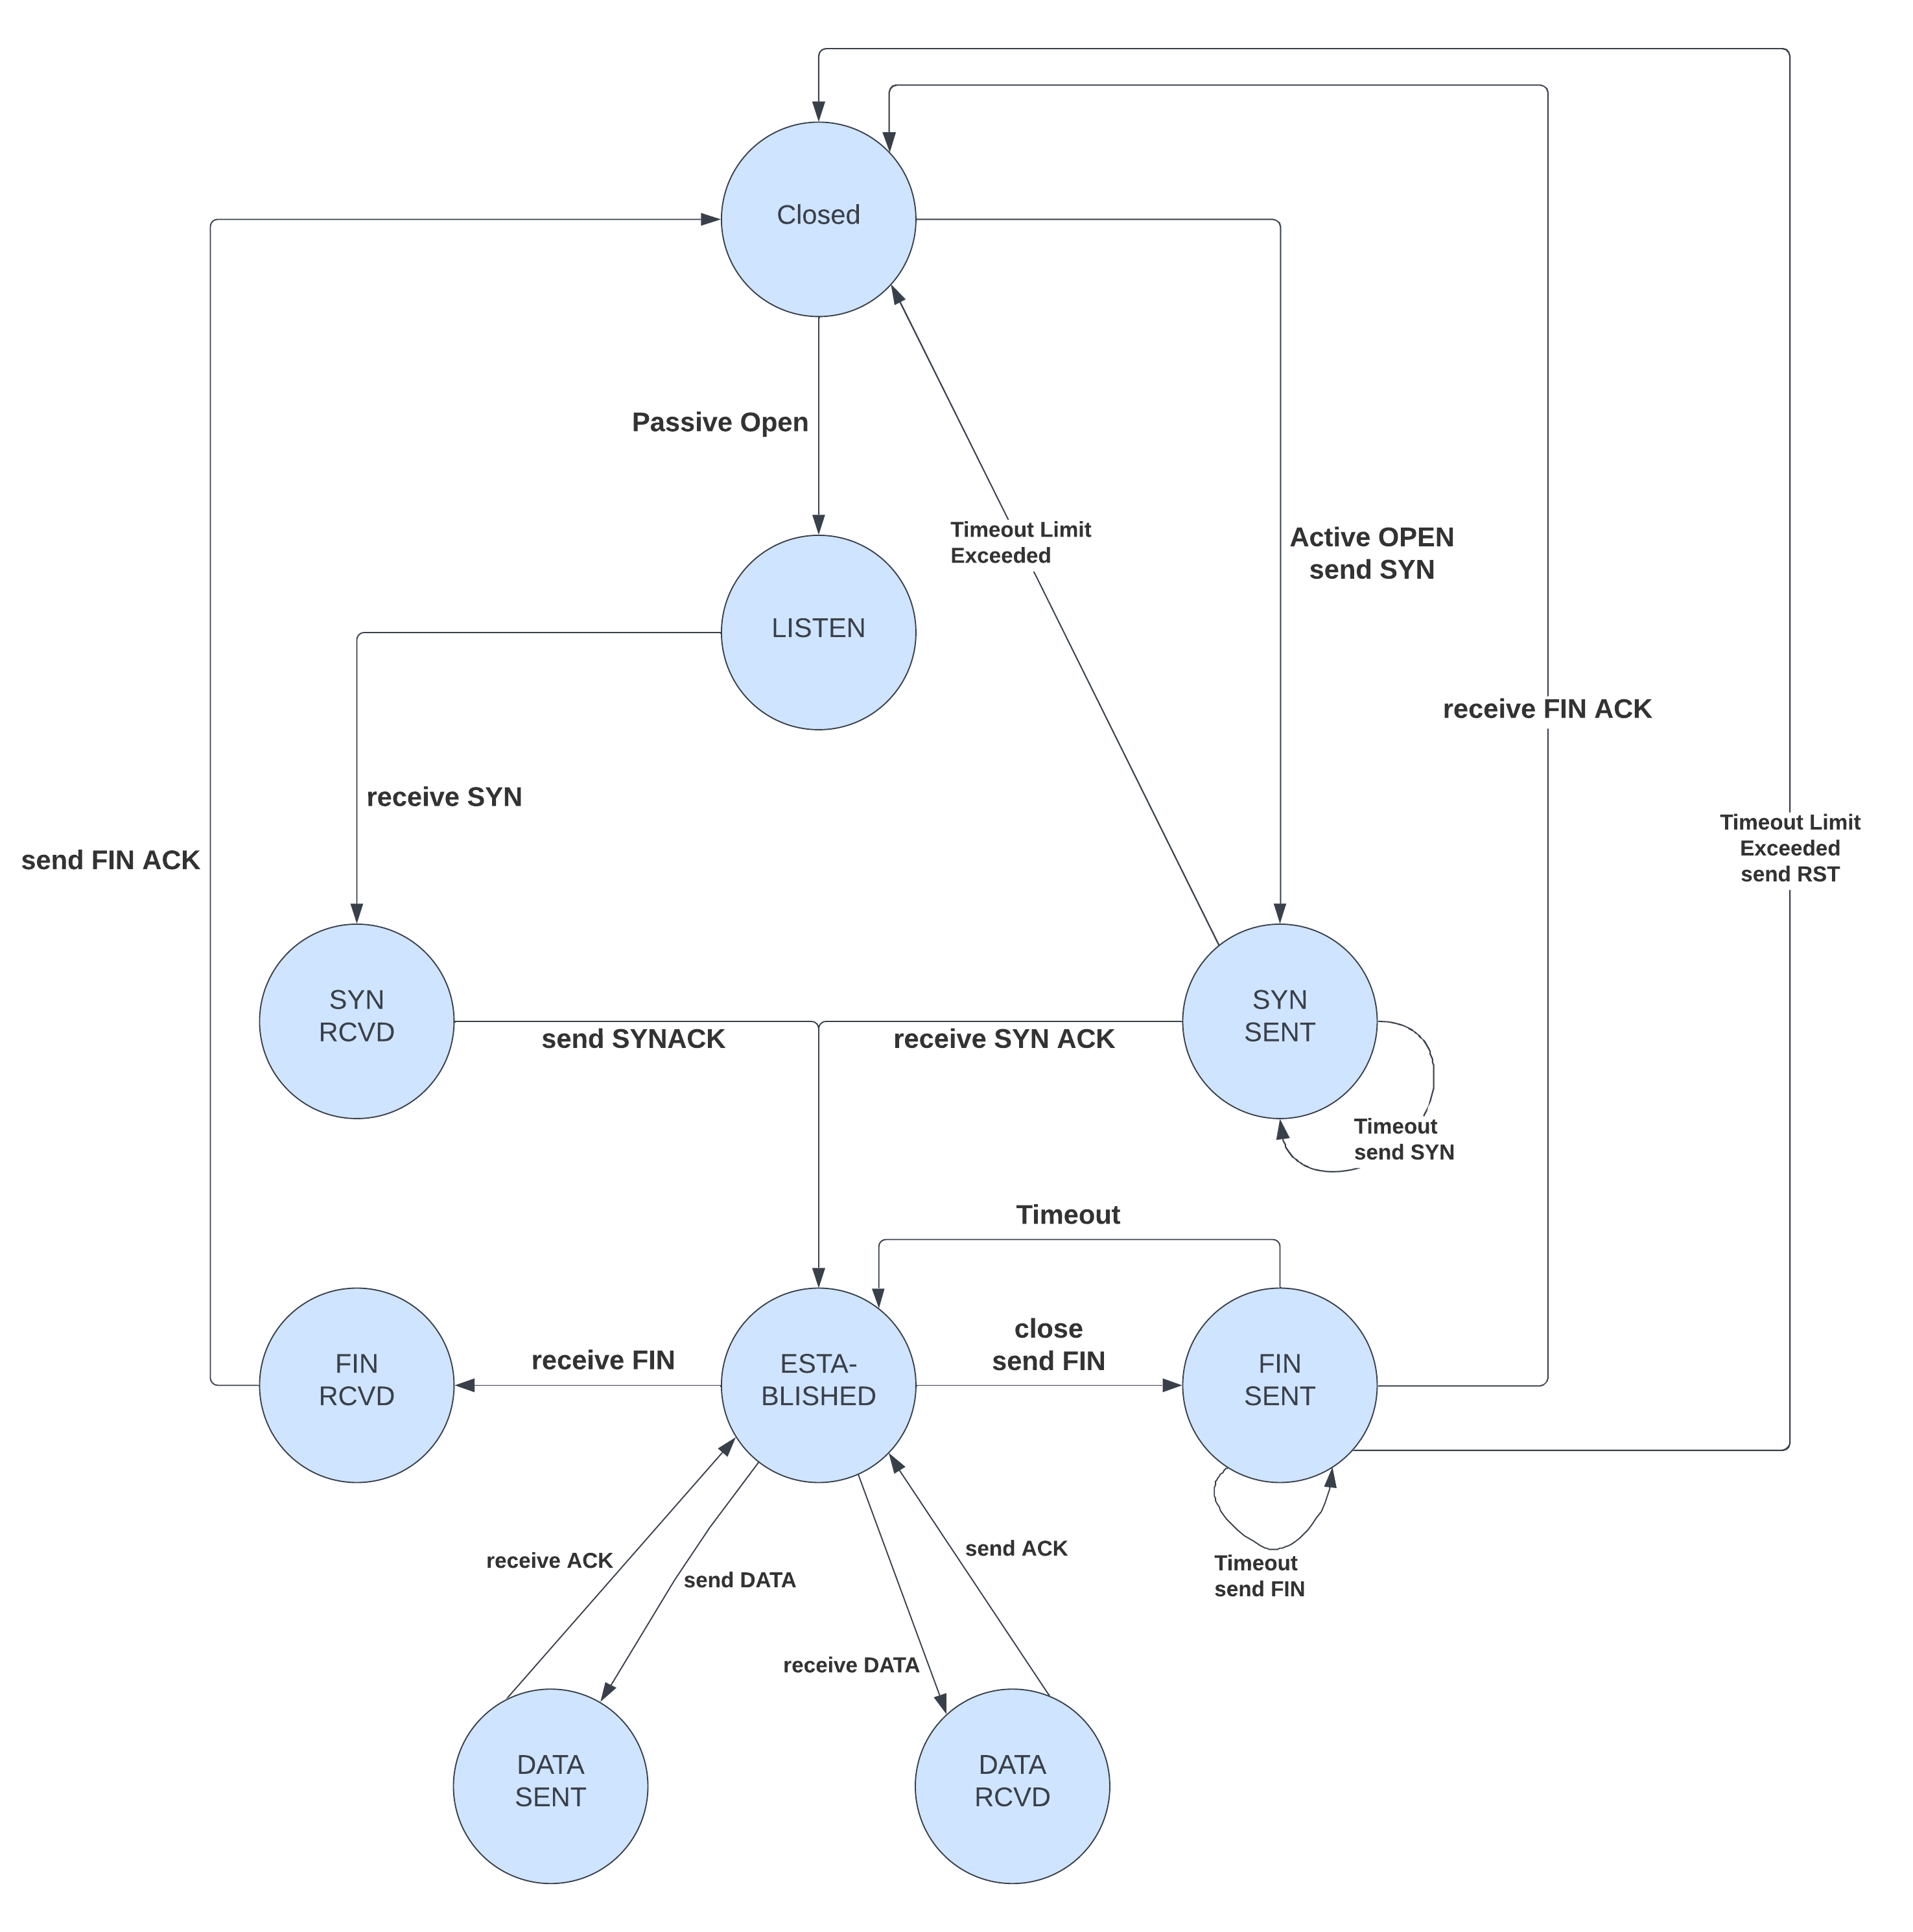
\includegraphics[width=100mm]{images/fsm.png}
\end{center}
\caption{RDT Finite State Machine (see also A.1)}\label{fig:fsm}
\end{figure}

\begin{figure}[h]
\begin{center}
    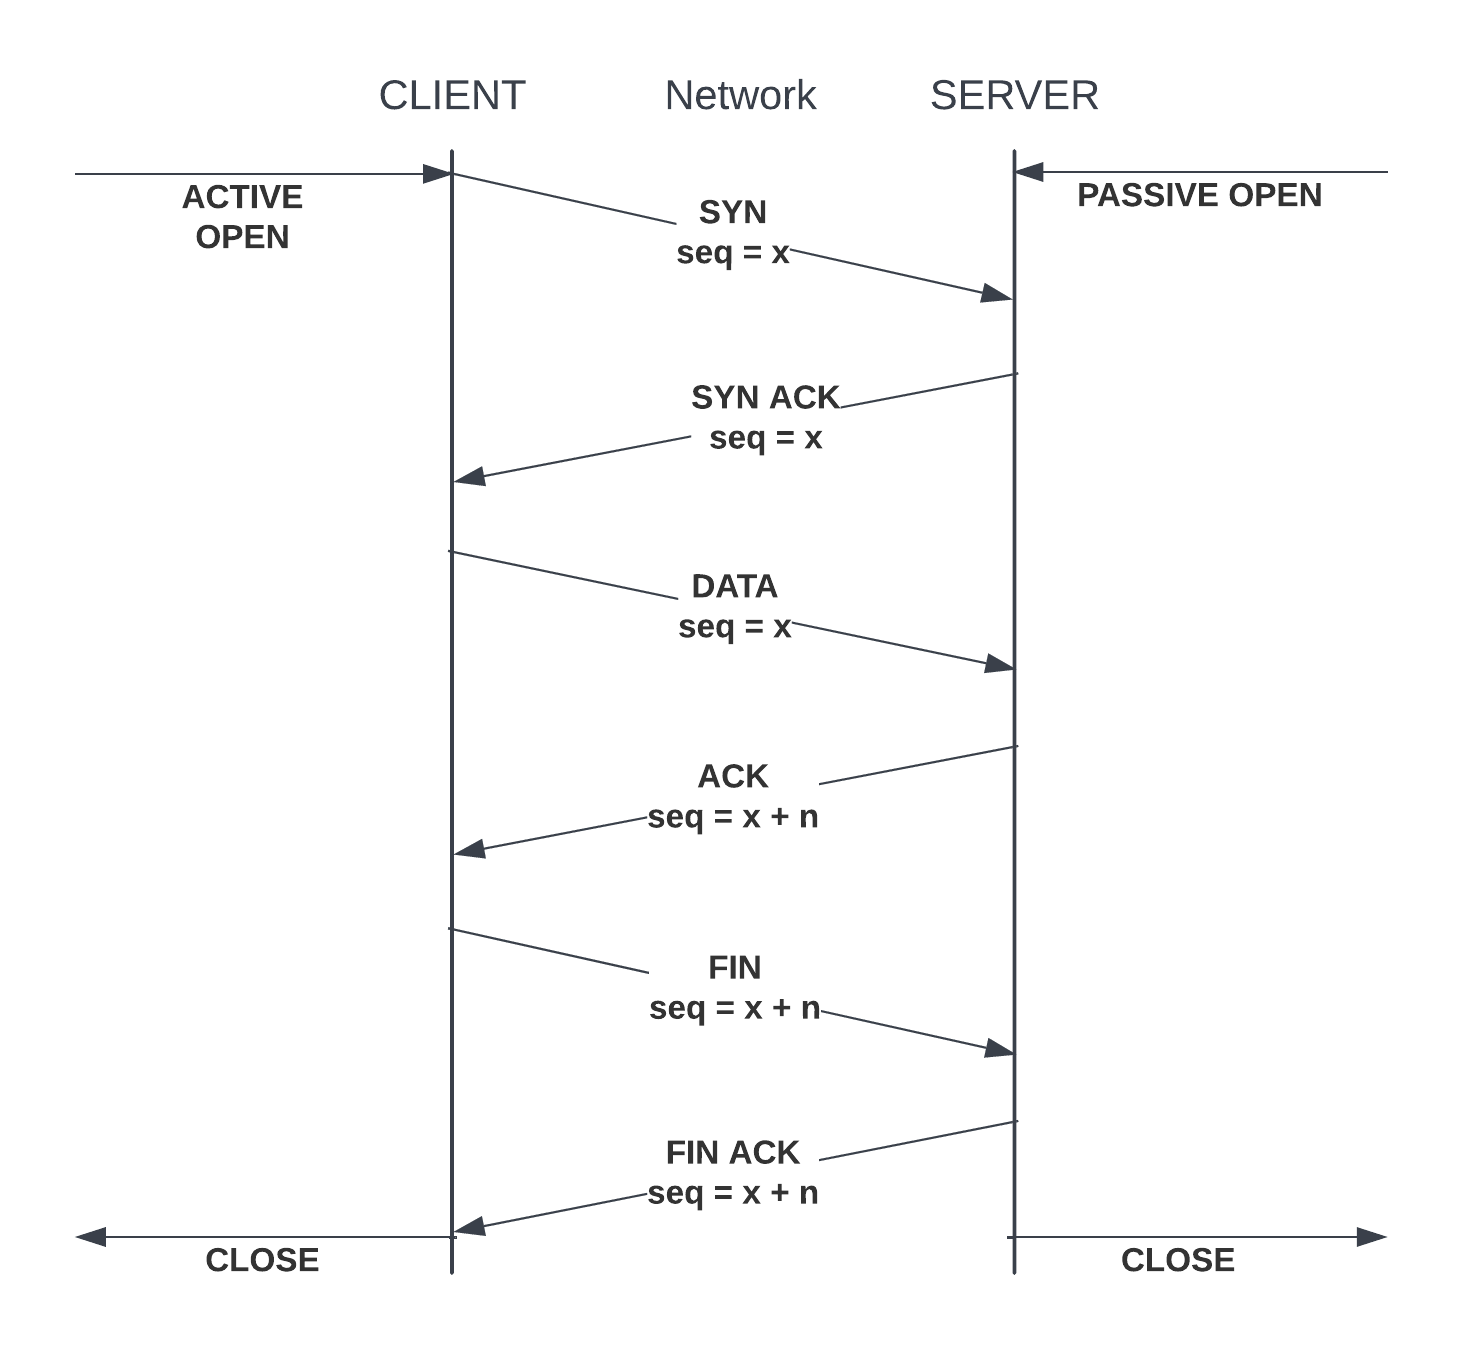
\includegraphics[width=100mm]{images/timeline.png}
\end{center}
\caption{Connection Timeline Diagram (see also A.2)}\label{fig:timeline}
\end{figure} 


\subsection{Checksums}
The RDT \code{checksum} field is calculated over the entire segment/packet (i.e.~header and data) using the IPv4 Header Checksum Algorithm~\cite{rfc791}. The implementation of the original source~\cite{ipv4_checksum} to support the use of 8-bit byte values in the data segment. During checksum calculating, the \code{checksum} field itself is set to 0 for consistency.

\section{Testing}

This section will detail how RDT was tested to validate correct operation.

\subsection{Methodology}

To test the ability of RDT to deliver packets in a reliable and ordered manner, two test programs were created. The latter was run on \textbf{pc} and the former on \textbf{pc}. Slurpe was place in the middle. A file was transmitted from A to B. Decoded with SHA.


\section{Analysis}

\subsection{Performance in Different Network Scenarios}
\label{sec:performance}

\begin{figure}[H]
\begin{center}
    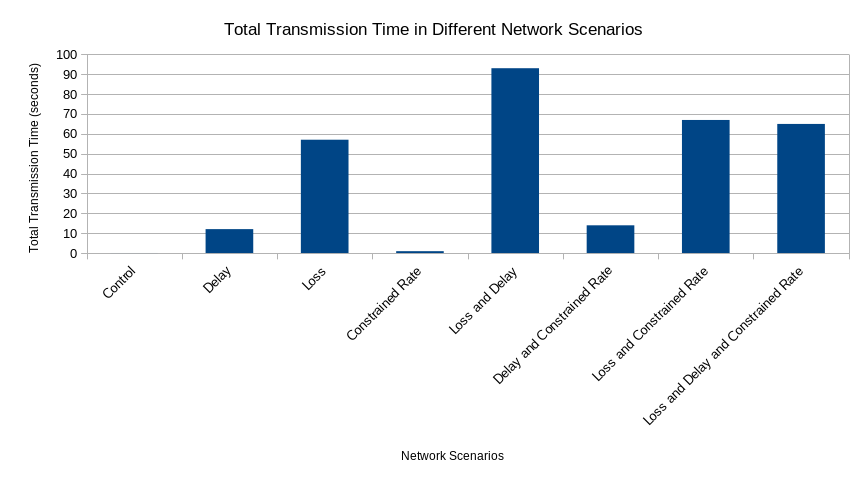
\includegraphics[width=100mm]{images/performance-network-scenarios.png}
\end{center}
\caption{Total Transmission Time in Different Network Scenarios for 230 Kb file.}\label{fig:performance}
\end{figure}

From Figure \ref{fig:performance} we can see that the network characteristic that has the biggest impact on the performance RDT is packet loss. 

\subsection{Bandwidth Delay Product and Link Utilisation}

The Bandwith-Delay Product (BDP) for a link represents the \textbf{what?} and is calculated as:

\begin{align*}
    BDP = \text{Bandwidth (bits per second)} \times \text{Round Trip Time (seconds)}
\end{align*}

For the link between \textbf{pcs} the observed average RTT with RDT was \textbf{RTT average}. This therefore yields a BDP of \textbf{BDP}.

As RDT only sends $1300 \text{\;bytes} = 10400 \text{\;bits}$ in each packet, this means that RDT achieves a link utilisation of $1040 / BDP = $.

\subsection{Maximum Theoretical Data Rate}



\subsection{Idle-RQ Performance}

\begin{align*}
    U_{RDT_IRQ} = \frac{N_pT_x}{T_x + 2T_p}
\end{align*}

where:
\begin{itemize}
    \item $N_p$ is the number of packets sent
    \item $T_x$ is the tranmission delay
    \item $T_p$ is the propogation delay
\end{itemize}

\subsection{RDT Packet Data Size}


\subsection{Wastage due to Control Information}

\begin{align*}
    \rho = \frac{i - c}{i + a} = \frac{1312 - 12}{1312 + 12} = 0.982 \text{\:(3 s.f.)}
\end{align*}

\section{Evaluation}
\subsection{Extension Features}

Given that RDT is implemented using UDP and uses the same checksum algorithm used by UDP, it is unlikley that RDT will ever encounter an incorrect checksum. This makes the use of a checksum in RDT mostly redundant. However the inclusion of a checksum provided some utility. Firstly, it helped to catch several errors in the initial implementation of RDT, and secondly it provided a useful. opportunity to understand the function of the Internet Checksum.

The inclusion of adaptive RTO was more useful however. From our analysis in Section \ref{sec:performance}, we concluded that the amount of retransmission required has the biggest impact on RDT performance. Whilst RDT do anything to minimise packet, it is able to control the number of retransmissions due to RTO via the adaptive RTO mechanism. Using the adaptive RTOs, RDT can account for varying amounts of network delay. Therefore we can say that adaptive RTO has had a positive impact on the efficiency and performance RDT in scenarios where network delay is present.

\subsection{Further Extension}

While the implementation of bi-directional communication and Continuous-RQ was not implemented, it is useful to consider these features in evaluating the desing of RDT.

In it's current design, RDT would be unable to support simulatenous bi-directional communication, due to its use of a two-way handshake. For bi-directional communication to occur, both parties are required to choose and synchronise an 'Initial Sequence Number', which is not possible with only a two-way handshake. Therefore, to support bi-directional communication RDT would require a significant re-design.

However, RDT would not require a fundamental re-design to support Continous-RQ. Continous-RQ with Go-Back-N would solve RDT's fundamental issue of low transmission rate due to link under-utilisation (see \textbf{section}).

\input{Conclusion}

\theendnotes
\newpage
\bibliographystyle{plain}
\bibliography{refs}

\newpage
\appendix{}
\section{Appendix}

\subsection{Finite State Machine}

\begin{figure}[H]
\begin{center}
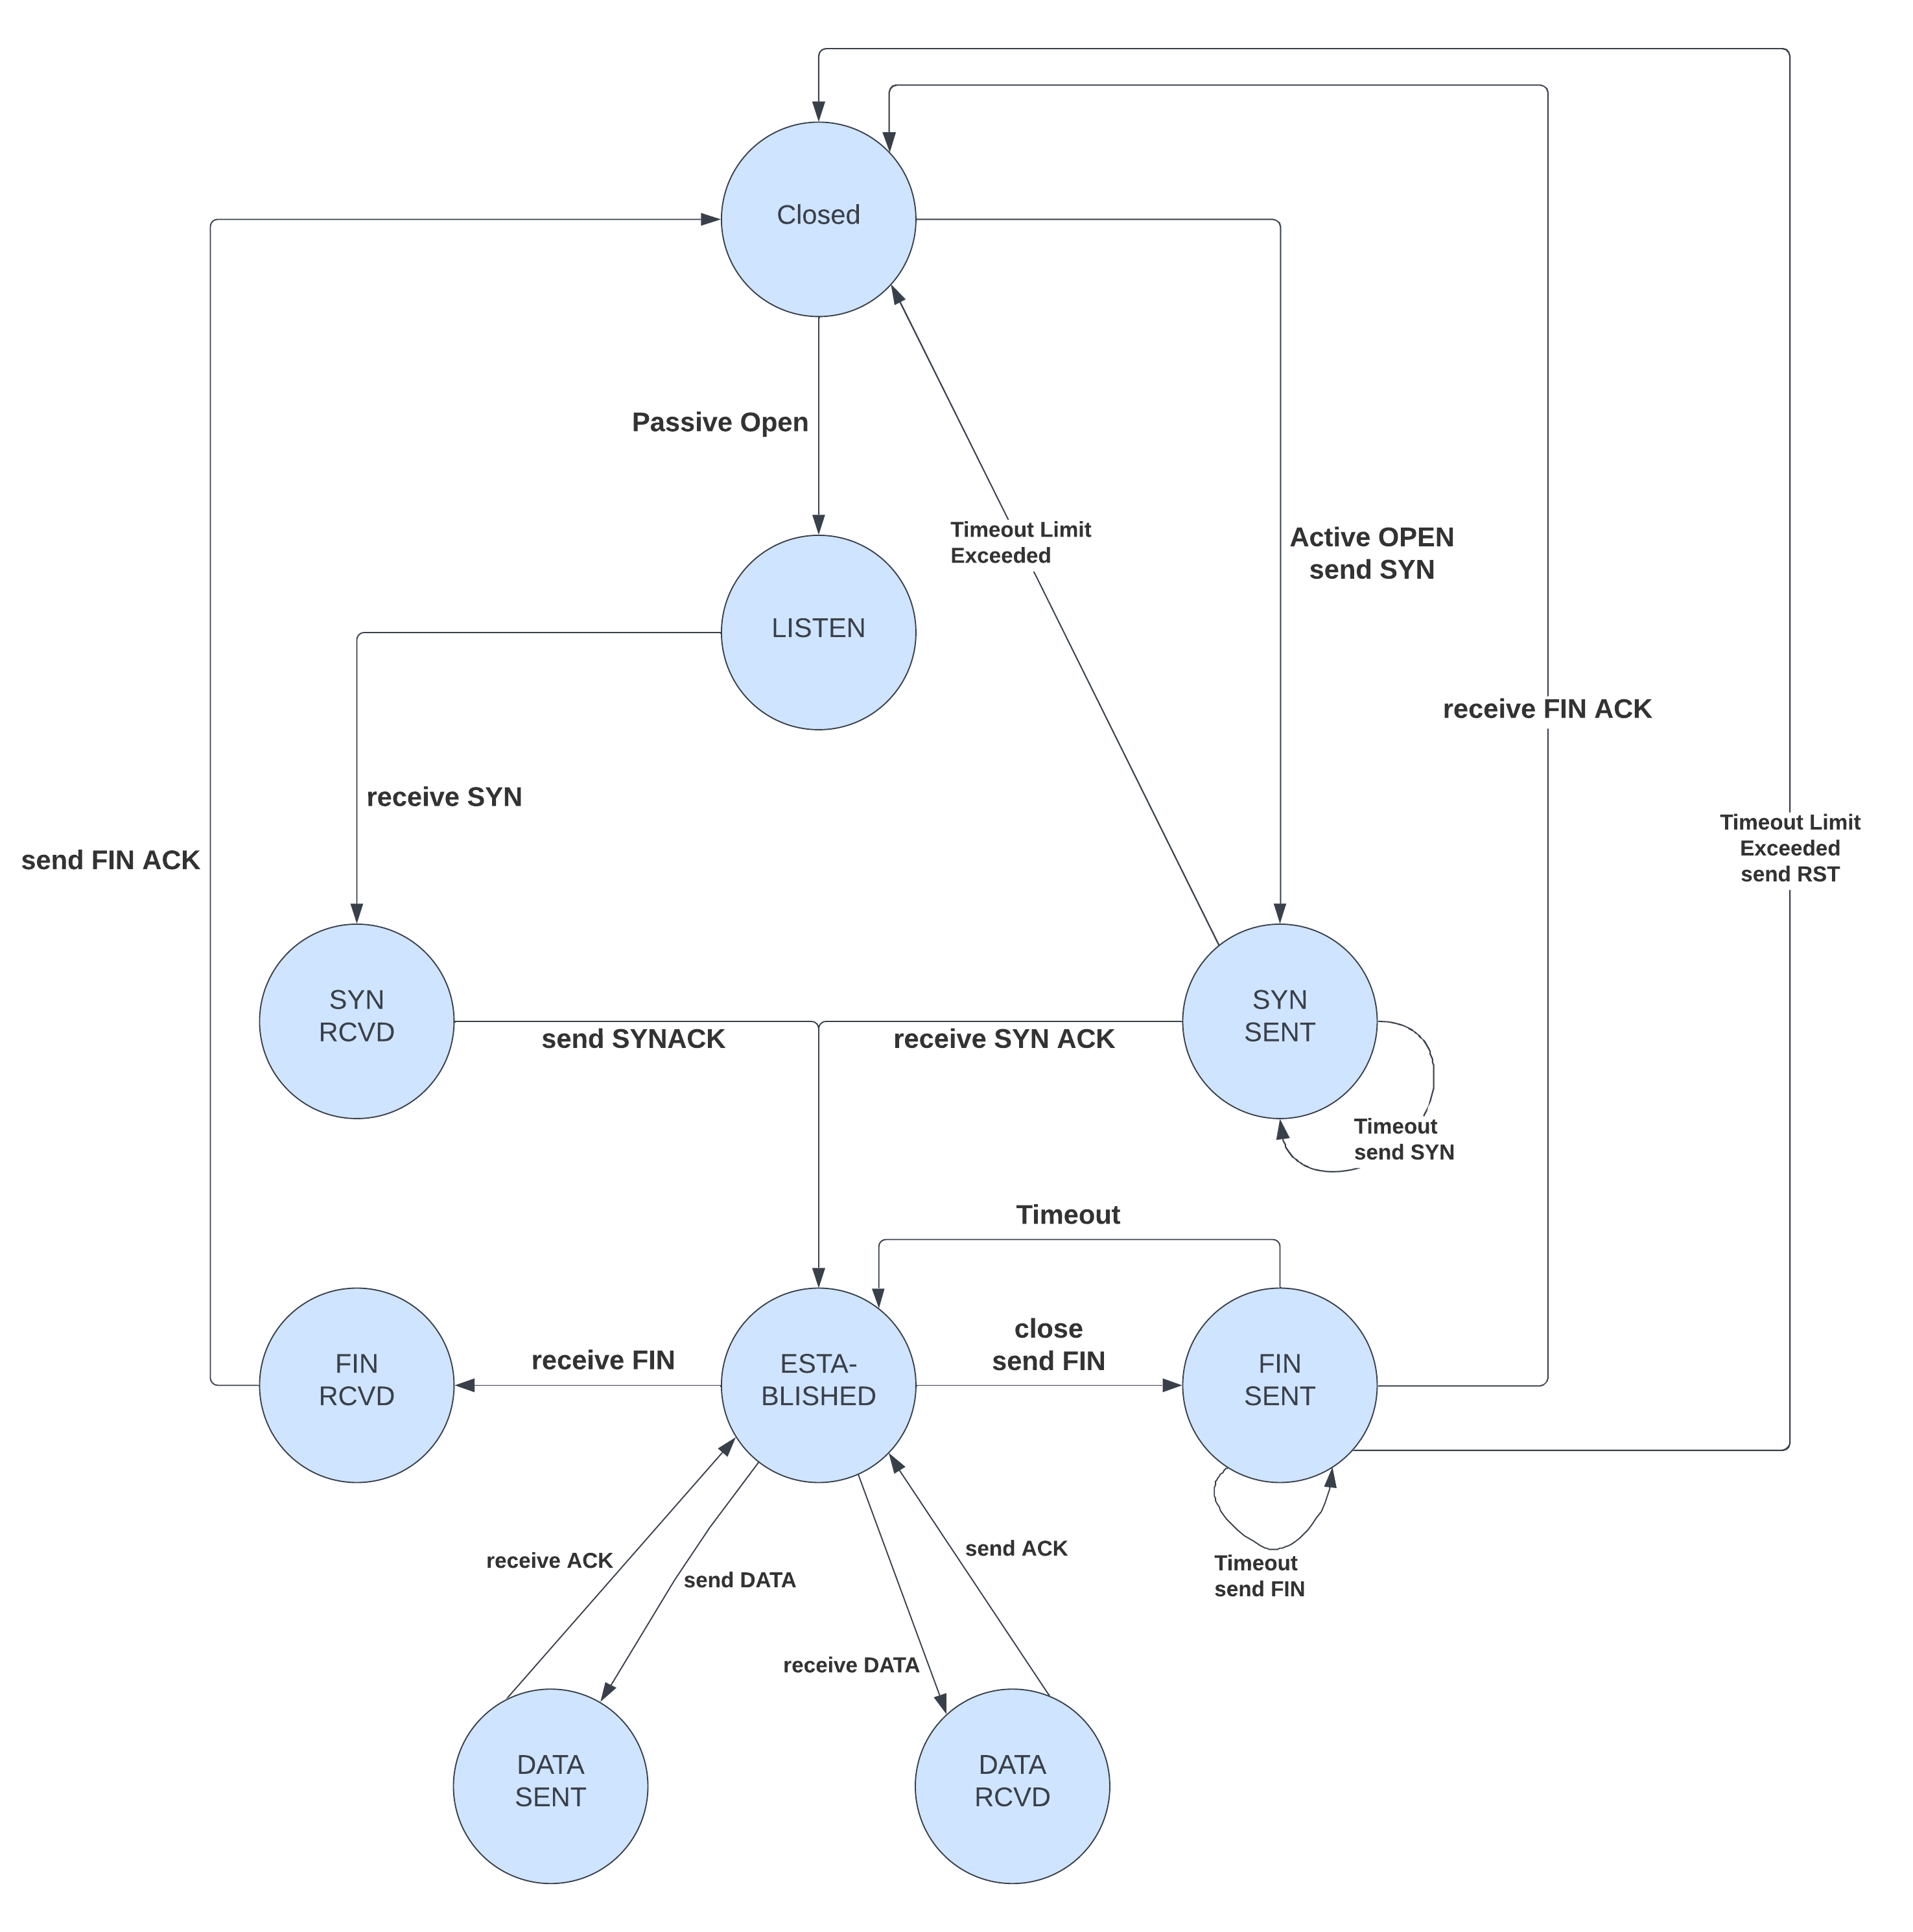
\includegraphics[width=170mm]{images/fsm.png}
\end{center}
\begin{center}
    Figure 3: RDT Finite State Machine
\end{center}
\end{figure}


\subsection{Connection Management Timeline Diagram}
\begin{figure}[H]
\begin{center}
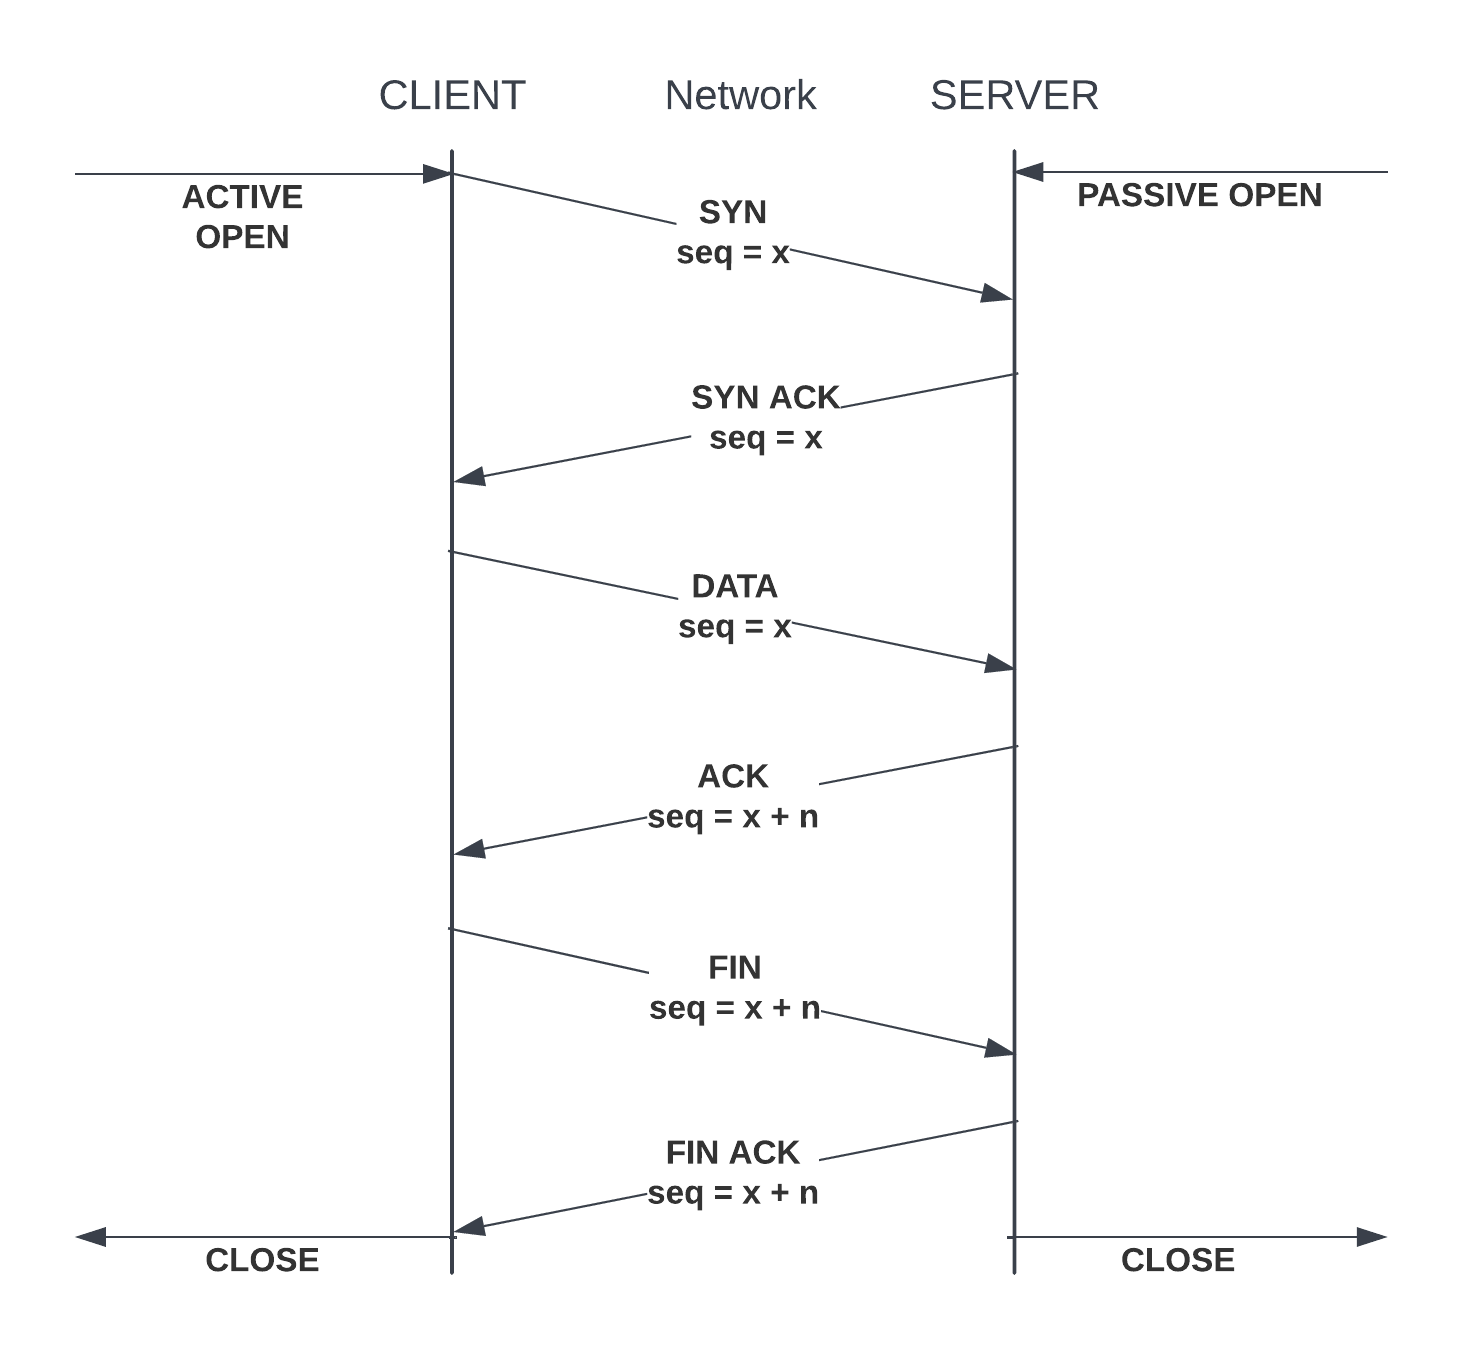
\includegraphics[width=170mm]{images/timeline.png}
\end{center}
\begin{center}
    Figure 4: Connection Timeline Diagram
\end{center}
\end{figure}


\subsection{Performance in Different Network Scenarios}
\begin{figure}[H]
\begin{center}
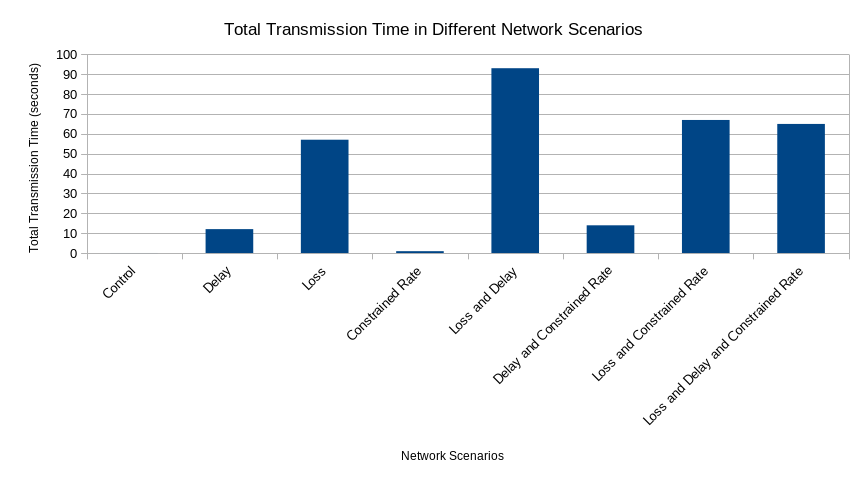
\includegraphics[width=170mm]{images/performance-network-scenarios.png}
\end{center}
\begin{center}
    Figure 5: Total Transmission Time in Different Network Scenarios for 230 Kb file.        
\end{center}
\end{figure}

\newpage
\subsection{Testing Screenshots}
\label{testing-screenshots}
Testing screenshots can be found inside the \code{data/screenshots} directory.

\end{document}